\documentclass[a4paper]{article}
\usepackage[a4paper,  margin=1.0in]{geometry}

\usepackage{graphicx}
\usepackage{float}
\usepackage{hyperref}
\usepackage{listings}
\lstset{
basicstyle=\small\ttfamily,
columns=flexible,
breaklines=true
}

\usepackage{polski}
\usepackage[utf8]{inputenc}
\begin{document}


\title{Ćwiczenie nr 2 z MBI, adnotacja DNA}
\author{Mateusz Chydziński, Michał Sypetkowski}
\maketitle

\section{Ogólne informacje}
Repozytorium git: \url{https://github.com/msypetkowski/MBI-exercises.git}.
W katalogu \texttt{cw2} repozytorim zawiera skrypty/polecenia użyte do przeprowadzenia eksperymentów.

\section{Przygotowanie danych}
W doświadczeniu wykorzystany został genom tasiemca (hymenolepis diminuta).
Cały ten genom (wyniki jego assemblingu) zawiera 3035 kontigów fizycznych (scaffolds).
Do badań wykorzystany został kontig fizyczny o identyfikatorze:
\begin{verbatim}
>HDID_scaffold0000001 length=355889
\end{verbatim}

\section{Maskowanie genomu}
% RepeatMasker is a program that screens DNA sequences for interspersed
% repeats and low complexity DNA sequences. The output of the program is
% a detailed annotation of the repeats that are present in the query
% sequence as well as a modified version of the query sequence in which
% all the annotated repeats have been masked (default: replaced by
% Ns). Sequence comparisons in RepeatMasker are performed by the program
% cross_match, an efficient implementation of the Smith-Waterman-Gotoh
% algorithm developed by Phil Green, or by WU-Blast developed by Warren
% Gish.

Program RepeatMasker maskuje sekwencje DNA pod względem powtórzeń oraz sekwencji DNA o niskiej złożoności.
Sekwencje są porównywane algorytmem Smitha-Watermana-Gotoha (zoptymalizowana wersja algorytmu Smitha-Watermana).
Wyjście programu to przede wszystkim:
\begin{itemize}
    \item sekwencja wejściowa, z zamaskowanymi powtórzeniami (plik .masked).
             Powtórzone podsekwencjie zostają zastąpione literami N.
    \item lista zamaskowanych powtórzeń z ich annotacjami.
            (plik .out).
            Adnotacje zawierają między innymi informację o powodzie uznania sekwencji za powtórzenie
            (niska złożoność sekwencji lub proste powtórzenie).
\end{itemize}

W naszym eksperymencie, ilość nukleotydów która została zamaskowana w wyniku działania programu to 2478.

\section{Mapowanie znanych sekwencji i adnotacja strukturalna}

% MAKER is a program that produces gene annotations in GFF3 format using
% evidence such as EST alignments and protein homology. MAKER can be used to
% produce gene annotations for new genomes as well as update annotations
% from existing genome databases.

Program maker na podstawie otrzymanej sekwencji z zamaskowanymi powtórzeniami
oraz danych białek i mRNA, tworzy adnotacje strukturalne genów w formacie GFF3.
Pierwsze 10 linii z logu programu maker:
\begin{lstlisting}
##gff-version 3
HDID_scaffold0000001	.	contig	1	355889	.	.	.	ID=HDID_scaffold0000001;Name=HDID_scaffold0000001
###
HDID_scaffold0000001	repeatmasker	match	7846	9011	1224	+	.	ID=HDID_scaffold0000001:hit:0:1.3.0.0;Name=species:Mariner-6_ACe|genus:DNA%2FTcMar-Tc1;Target=species:Mariner-6_ACe|genus:DNA%2FTcMar-Tc1 1 1094 +
HDID_scaffold0000001	repeatmasker	match_part	7846	9011	1224	+	.	ID=HDID_scaffold0000001:hsp:0:1.3.0.0;Parent=HDID_scaffold0000001:hit:0:1.3.0.0;Target=species:Mariner-6_ACe|genus:DNA%252FTcMar-Tc1 1 1094 +
HDID_scaffold0000001	repeatmasker	match	42975	43896	707	+	.	ID=HDID_scaffold0000001:hit:1:1.3.0.0;Name=species:Mariner-6_CFl|genus:DNA%2FTcMar-Mariner;Target=species:Mariner-6_CFl|genus:DNA%2FTcMar-Mariner 262 1175 +
HDID_scaffold0000001	repeatmasker	match_part	42975	43896	707	+	.	ID=HDID_scaffold0000001:hsp:1:1.3.0.0;Parent=HDID_scaffold0000001:hit:1:1.3.0.0;Target=species:Mariner-6_CFl|genus:DNA%252FTcMar-Mariner 262 1175 +
HDID_scaffold0000001	repeatmasker	match	162805	163521	673	+	.	ID=HDID_scaffold0000001:hit:2:1.3.0.1;Name=species:Mariner-43_HSal|genus:DNA%2FTcMar-Mariner;Target=species:Mariner-43_HSal|genus:DNA%2FTcMar-Mariner 494 1199 +
HDID_scaffold0000001	repeatmasker	match_part	162805	163521	673	+	.	ID=HDID_scaffold0000001:hsp:2:1.3.0.1;Parent=HDID_scaffold0000001:hit:2:1.3.0.1;Target=species:Mariner-43_HSal|genus:DNA%252FTcMar-Mariner 494 1199 +
HDID_scaffold0000001	repeatmasker	match	163678	163840	231	+	.	ID=HDID_scaffold0000001:hit:3:1.3.0.1;Name=species:Mariner-25_HSal|genus:DNA%2FTcMar-Mariner;Target=species:Mariner-25_HSal|genus:DNA%2FTcMar-Mariner 185 347 +
\end{lstlisting}

Przykładowa annotacja typu \texttt{expressed\_sequence\_match} w pliku .gff (wygenerowanego przez program maker):
\begin{lstlisting}
HDID_scaffold0000001	blastn	expressed_sequence_match	17669	18426	40	-	.	ID=HDID_scaffold0000001:hit:16:3.2.0.0;Name=HDID_0000675501-mRNA-1
\end{lstlisting}

Źródłem tej annotacji jest program blastn, zwracający najbardziej podobne sekwencje DNA z bazy danych.
W naszym przypadku bazą danych jest plik z sekwencją mRNA (zbiorem scaffoldów) dla tasiemca
(sekwencja została dopasowana do scaffolda o identyfikatorze \texttt{HDID\_0000675501-mRNA-1}).


Nukleotydy w tej sekwencji to:

\begin{verbatim}
TTAAAATCCAGAACAACAAGCCTTTTTCGGTTGGTTACTGTCCTGTTGGAGAGGAATAGT
AGGCTTACTGCCCAATGGAAGGGCATTATTGGAATTCACGGAGGGTGTTCCTACAATTTT
AAGAATATCTTAACAAAAATCGCACTTGAAAAGTAGTCCTTACCTTCAAGAAGGGTGGAA
AAAGCTCGATCGACATTGGTTGAGTCTAAGGCTGATGTTTCAATGAAGTGAAGACAAGTA
TCTTCAGCGAATTGCTTGGCTTCTTGCGTAGAAACCGTACGCAGATGGCGCAGATCACAT
TTATTTCCAACTAATATGGTGACAATATTTCGATCAGCATTATTCTTAAGTTCCTTCAAC
CATACGTTCACATTTTCAAAAGTAGTGTACTTAGCTATATCATATACAAGCAGAGCTCCA
ACAGCACCGCGATAATACCTATAGAAAACAGAACTAATTATAGAAAAATACTCAACTTAC
GCTGACGTTATTGCTCTGTATCTTTCTTGGCCGGCTGTATCCCAAATTTGGATTTTTATA
ACCTTATCACCTATCTTAACACTCCTGGTTGCGAATTCAACGCCGATTGTGGTTTTACTC
TCCAAGTTAAATTGATTACGAGTGTATCGAGAGAGTAGATTGCTCTTACCGACACCTGAA
TCCCCTATTAATACGACTAAAATATATAAGAAATGATTAATTAAAAGAAAATAAATACTT
TTGAAAAGGTAATCATATGAATCTTCATCGTTGGCCA
\end{verbatim}


\section{Adnotacja funkcjonalna}
Genom użyty w badaniu należy do organizmu \texttt{hymenolepis diminuta}, czyli tasiemca szczurzego.
Analiza podobieństwa sekwencji za pomocą algorytmu BlastX została przeprowadzaona dla scaffoldu pierwszego,
o oznaczeniu \texttt{HDID\_scaffold0000001}.

W wyniku działania algorytmu (rysunek \ref{fig:result}), zostały znalezione 4 sekwencje o znacznym stopniu podobieństwa
(94\% dla 1 sekwencji oraz 100\% dla 3 pozostałych -- w tym również dla badanej sekwencji tasiemca szczurzego).
Istotność wyniku \texttt{E-value} jest na poziomie około \texttt{0.004},
co spełnia warunek \texttt{E<<1} i sprawia, że prawdopobieństwo przypadkowego dopasowania
sekwencji źródłowej do znalezionych jest bardzo małe.

Pierwszy wynik na liście potwierdza, że jest to rzeczywiście poprawny scaffold tego organizmu
(stopień podobieństwa 100\% oraz E-value=0). Ponadto stwierdzono duży stopień podobieństwa sekwencji do \texttt{Candida dubliniensis} - odmiany
patogennego grzyba (sekwencja kodująca jedno z białek oraz chromosom nr.1). Ostatnim wpisem na liście wyników jest jedno z białek orgaznizmu
\texttt{chenopodium quinoa}, czyli rośliny - komosy ryżowej. 

\begin{figure}[h]
    \centering
    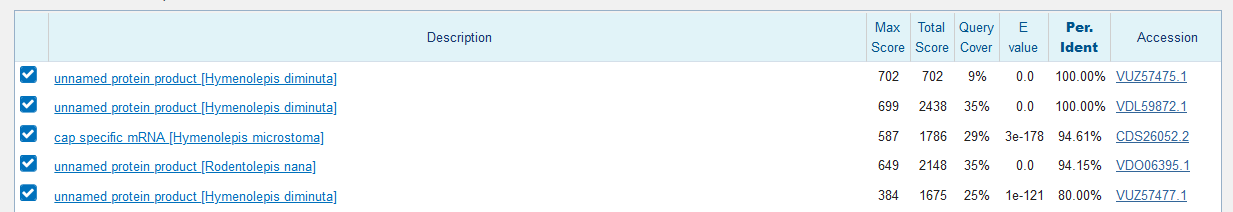
\includegraphics[width=1.0\textwidth]{result.png}
    \label{fig:result}
    \caption[]{Wyniki algorytmu BLASTX z bazy NCBI}
\end{figure}

\end{document}
